\chapter{Схемотехнический расчет СФ-блоков}

\section{Устройство выборки-хранения}
Определим мощность шумов квантования идеального АЦП с разрядностью \(N\) и размахом полной шкалы \(V_{FS}\)
\[ {P_{q}}^2 = \frac{\Delta^2}{12}\]
если \(\Delta = \dfrac{V_{FS}}{2^N}\), тогда \( {P_q}^2 = 223.52~\mathrm{pW} \).

\section*{Технические требования к аналого-цифровому преобразователю}
Характеристики приведены в Табл.~\ref{tab:Parameters}.
\begin{table}[h]
	\caption[Характеристики разрабатываемого АЦП]{Характеристики разрабатываемого АЦП}
	\label{tab:Parameters}
	\centering
	\begin{tabular}{rrr}
		\toprule
		\textbf{Параметр}      & \textbf{Значение} & \textbf{Единица измерения}\\
		\midrule
		\(N\)                 &   14      & Бит\\
		\(F_{clk}\)           &   250     & МГц\\
		\(V_{FS}\)            &   1.2     & В\\
		\(V_{CM_{in}}\)                   &   600     & мВ\\
		\(FPBW\) (Full Power Bandwidth)   & 750 & МГц\\
		\bottomrule
	\end{tabular}
\end{table}

УВХ построено на базе МОП ключа Q1 с цепью смещения напряжения затвора \(V_{gs1}\), позволяющей снизить нелинейность ключа, возникающую из-за неполного <<закрытия>> или <<открытия>> канала.

\begin{figure}[ht]
	\centering
	\includegraphics{Dissertation/images/tha.tikz}
	
	\caption{Схема устройства выборки-хранения}
	\label{ct:bootstrapped_switch}
\end{figure}

\begin{figure}[ht]
	\centering
	\includegraphics{Dissertation/images/lna_balun.tikz}
	
	\caption{Схема электрическая принципиальная рассматриваемого МШУ}
	\label{ct:lna_balun_wo_bias}
\end{figure}

\begin{figure}[ht]
	\centering
	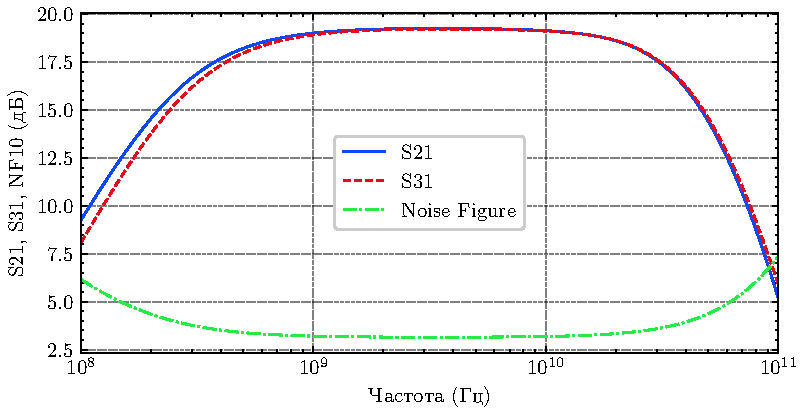
\includegraphics{lna_gain_nf.pdf}
	
	\caption{Коэффициенты усиления и шума рассматриваемого МШУ согласно результатам моделирования}
	\label{ct:lna_gain_nf}
\end{figure}

\begin{figure}[ht]
	\centering
	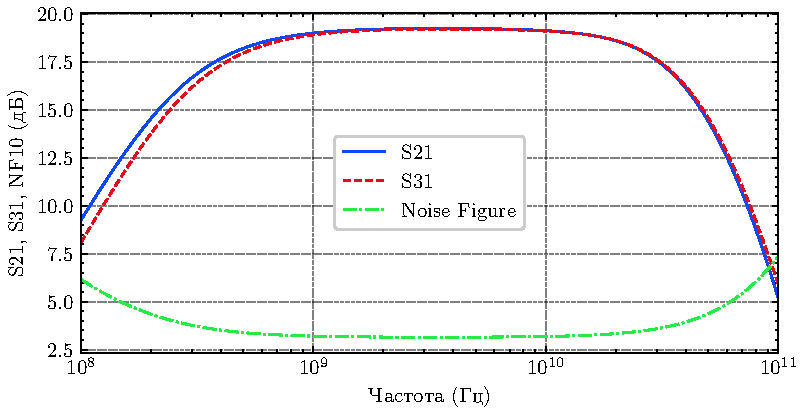
\includegraphics[width=6in,	height=3in]{lna_gain_nf.tikz}
	
	\caption{Коэффициенты усиления и шума рассматриваемого МШУ согласно результатам моделирования}
	\label{ct:lna_gain_tikz}
\end{figure}

\begin{figure}[ht]
	\centering
	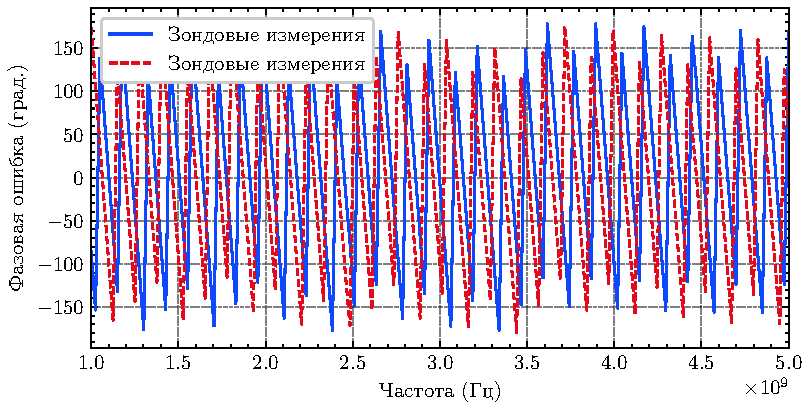
\includegraphics{probe_phase.pdf}
	
	\caption{Коэффициенты усиления и шума рассматриваемого МШУ согласно результатам моделирования}
	\label{ct:ps_phase}
\end{figure}

\begin{figure}[ht]
	\centering
	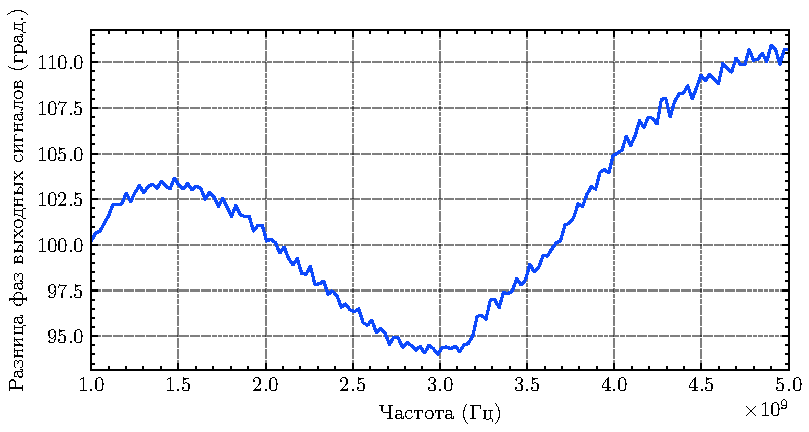
\includegraphics{probe_phase_error.pdf}
	
	\caption{Значение фазовой ошибки разработанного активного фазовращателя 1 - 2 ГГц}
	\label{ct:ps_phase_error}
\end{figure}

\begin{figure}[ht]
	\centering
	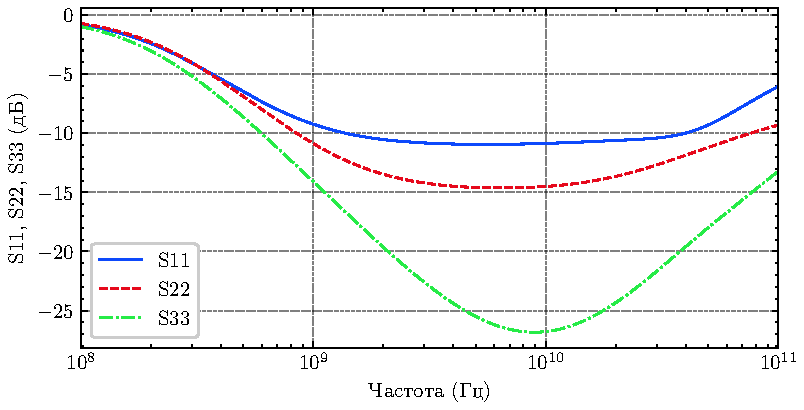
\includegraphics{lna_s11_s22.pdf}
	
	\caption{Результаты моделирования возвратных потерь по входу и выходу рассматриваемого МШУ}
	\label{ct:lna_s11_s22}
\end{figure}

\begin{figure}[ht]
	\centering
	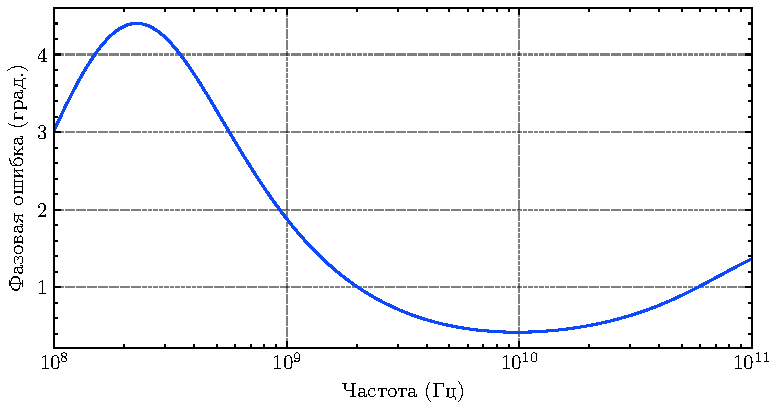
\includegraphics{phase_diff.pdf}
	
	\caption{Разница фаз между диффиренциальными компонентами на выходе рассматриваемого МШУ согласно результатам моделирования}
	\label{ct:phase_diff}
\end{figure}

\begin{figure}[ht]
	\centering
	\includegraphics{Dissertation/images/mixer.tikz}
	
	\caption{Схема электрическая принципиальная сверхширокополосного смесителя}
	\label{ct:mixer_1_18}
\end{figure}

\begin{figure}[ht]
	\centering
	\resizebox{\linewidth}{!}{\input{Dissertation/images/drawing.pdf_tex}}
	
	\caption{Схема структурная - pdf\_tex}
	\label{ct:drawing}
\end{figure}

\begin{figure}[ht]
	\centering
	\begin{circuitikz}[american, scale=1, transform shape]
		\def\killdepth#1{{\raisebox{0pt}[\height][0pt]{#1}}} \path (0,0) -- (2,0); % bounding box
		
		\ctikzset{bipoles/amp/width=1.2}
		\draw (0,0) to[amp,t=LNA,l_=$F{=}12\,$dB, o-] ++(4,0);
		
		%COOOOOORDS
		%\path (tmp) \coord(tmp);
	\end{circuitikz}
	
	\caption{Структурная схема тракта приемника МИЧ \numrange{1}{1.8} ГГц и \numrange{1.8}{3.3} ГГц}
	\label{ct:struct_1_8_3_3}
\end{figure}

\begin{figure}[ht]
	\centering
	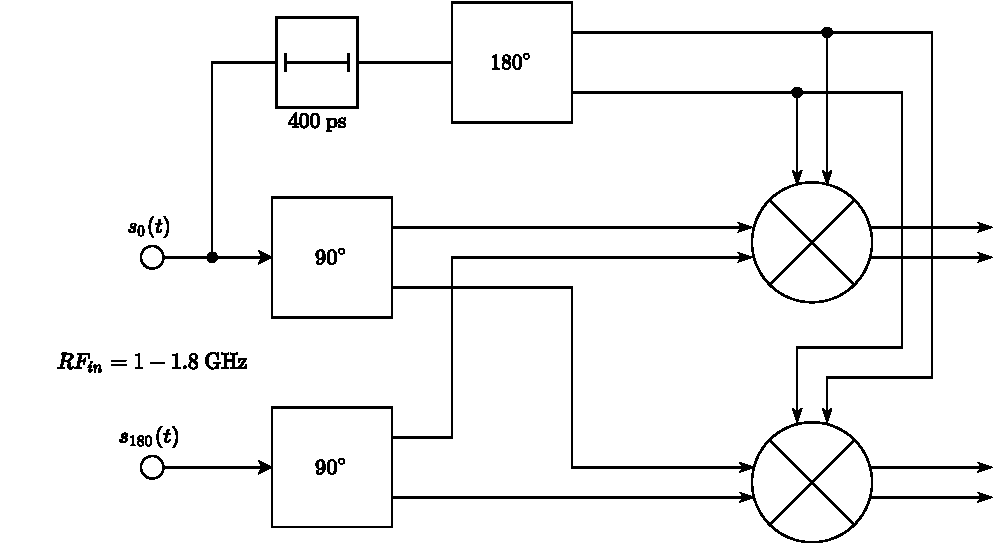
\includegraphics[width=0.6\linewidth]{IFM_Struct.pdf}
	
	\caption{Структурная схема частотного дискриминатора диапазона \numrange{1}{1.8} ГГц и \numrange{1.8}{3.3}}
	\label{ct:freq_estimate_1g_1g8}
\end{figure}

\begin{figure}[ht]
	\centering
	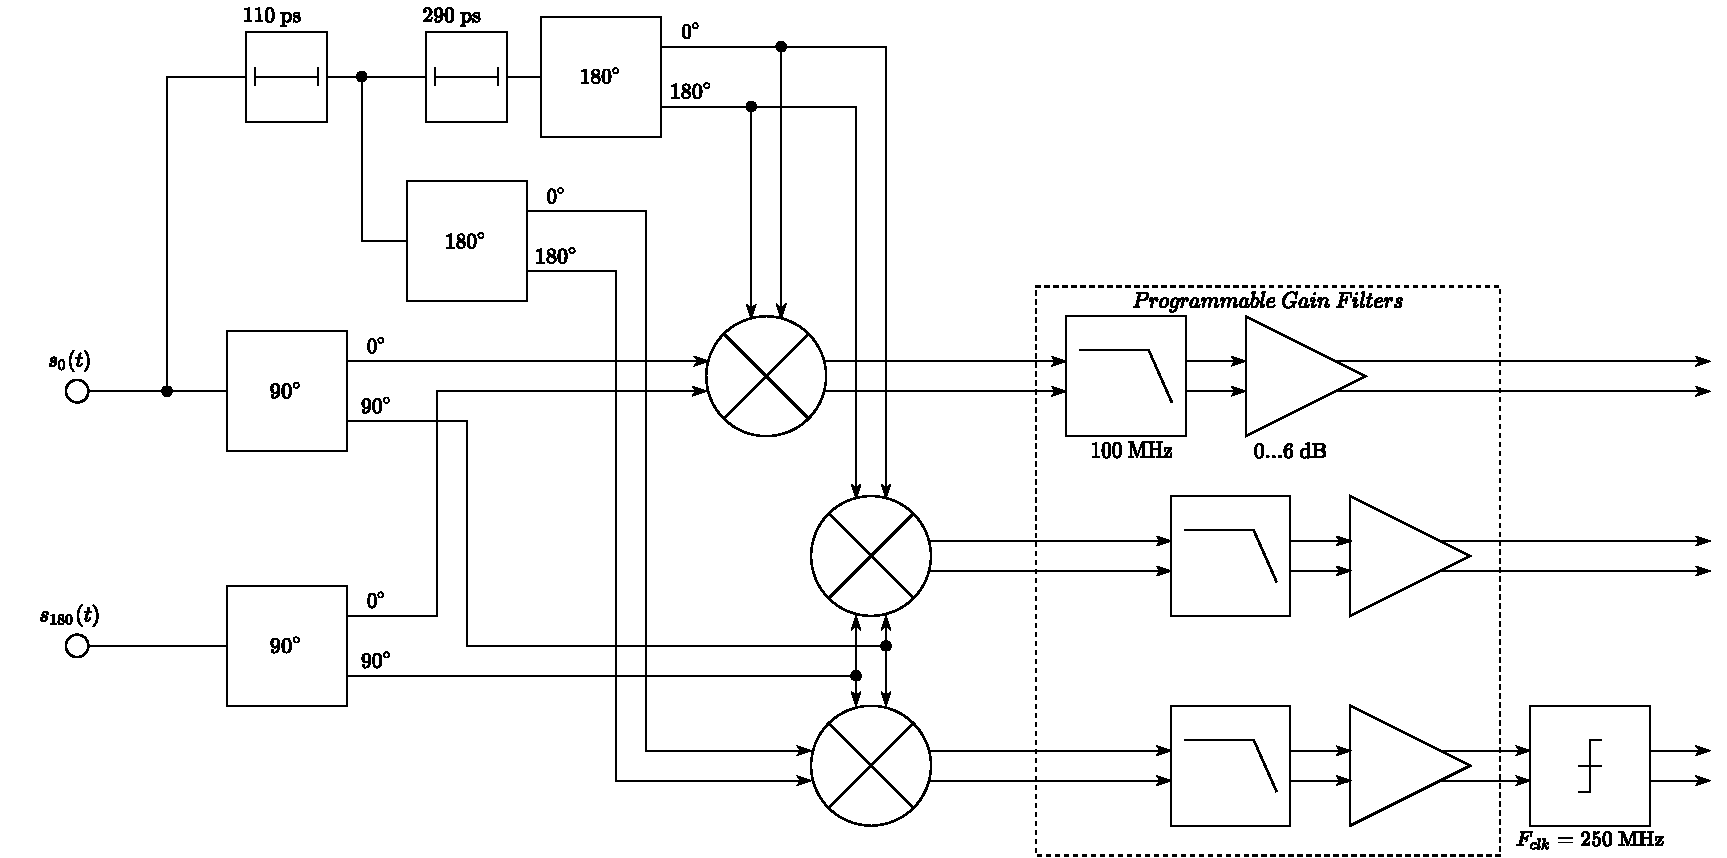
\includegraphics[width=1\linewidth]{IFM_Struct2.pdf}
	
	\caption{Структурная схема частотного дискриминатора диапазона \numrange{3.3}{6.3} ГГц}
	\label{ct:freq_estimate_3g3_6g3}
\end{figure}

\begin{figure}[ht]
	\centering
	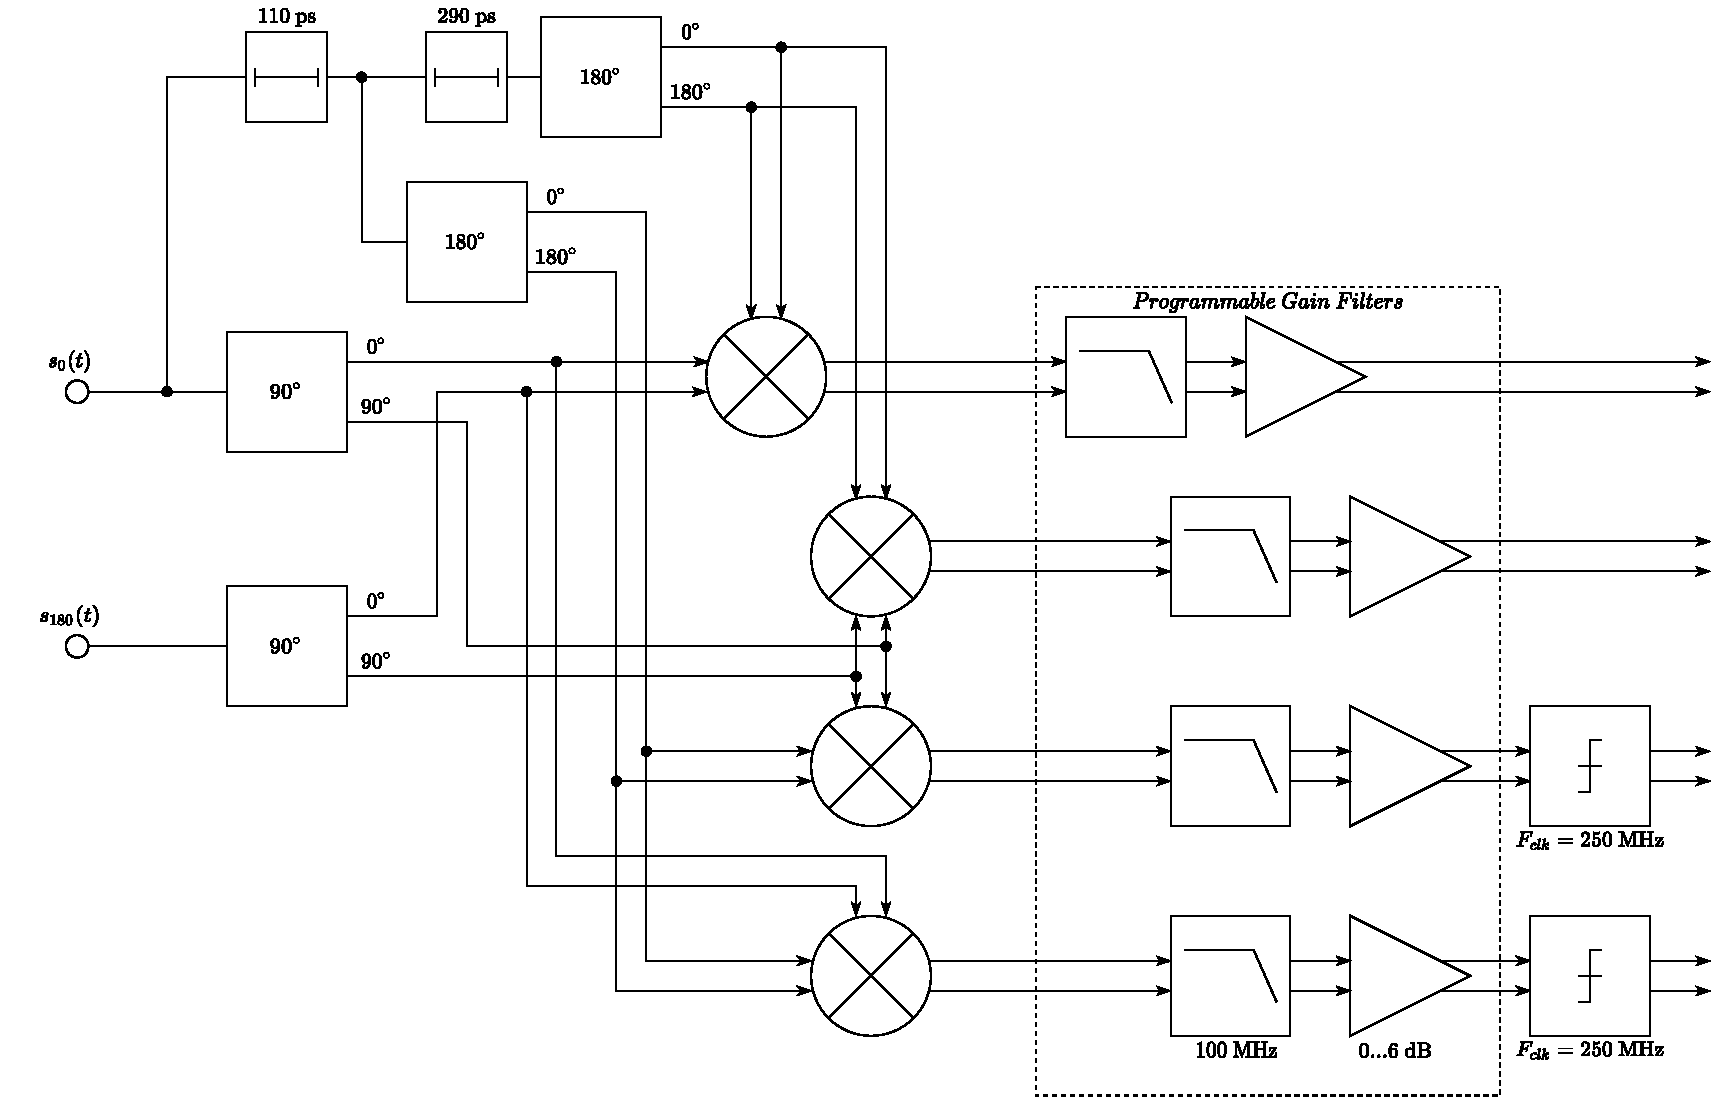
\includegraphics[width=1\linewidth]{IFM_Struct3.pdf}
	
	\caption{Структурная схема частотного дискриминатора диапазона \numrange{6.3}{11.5} ГГц}
	\label{ct:freq_estimate_6g3_12g}
\end{figure}

\begin{figure}[ht]
	\centering
	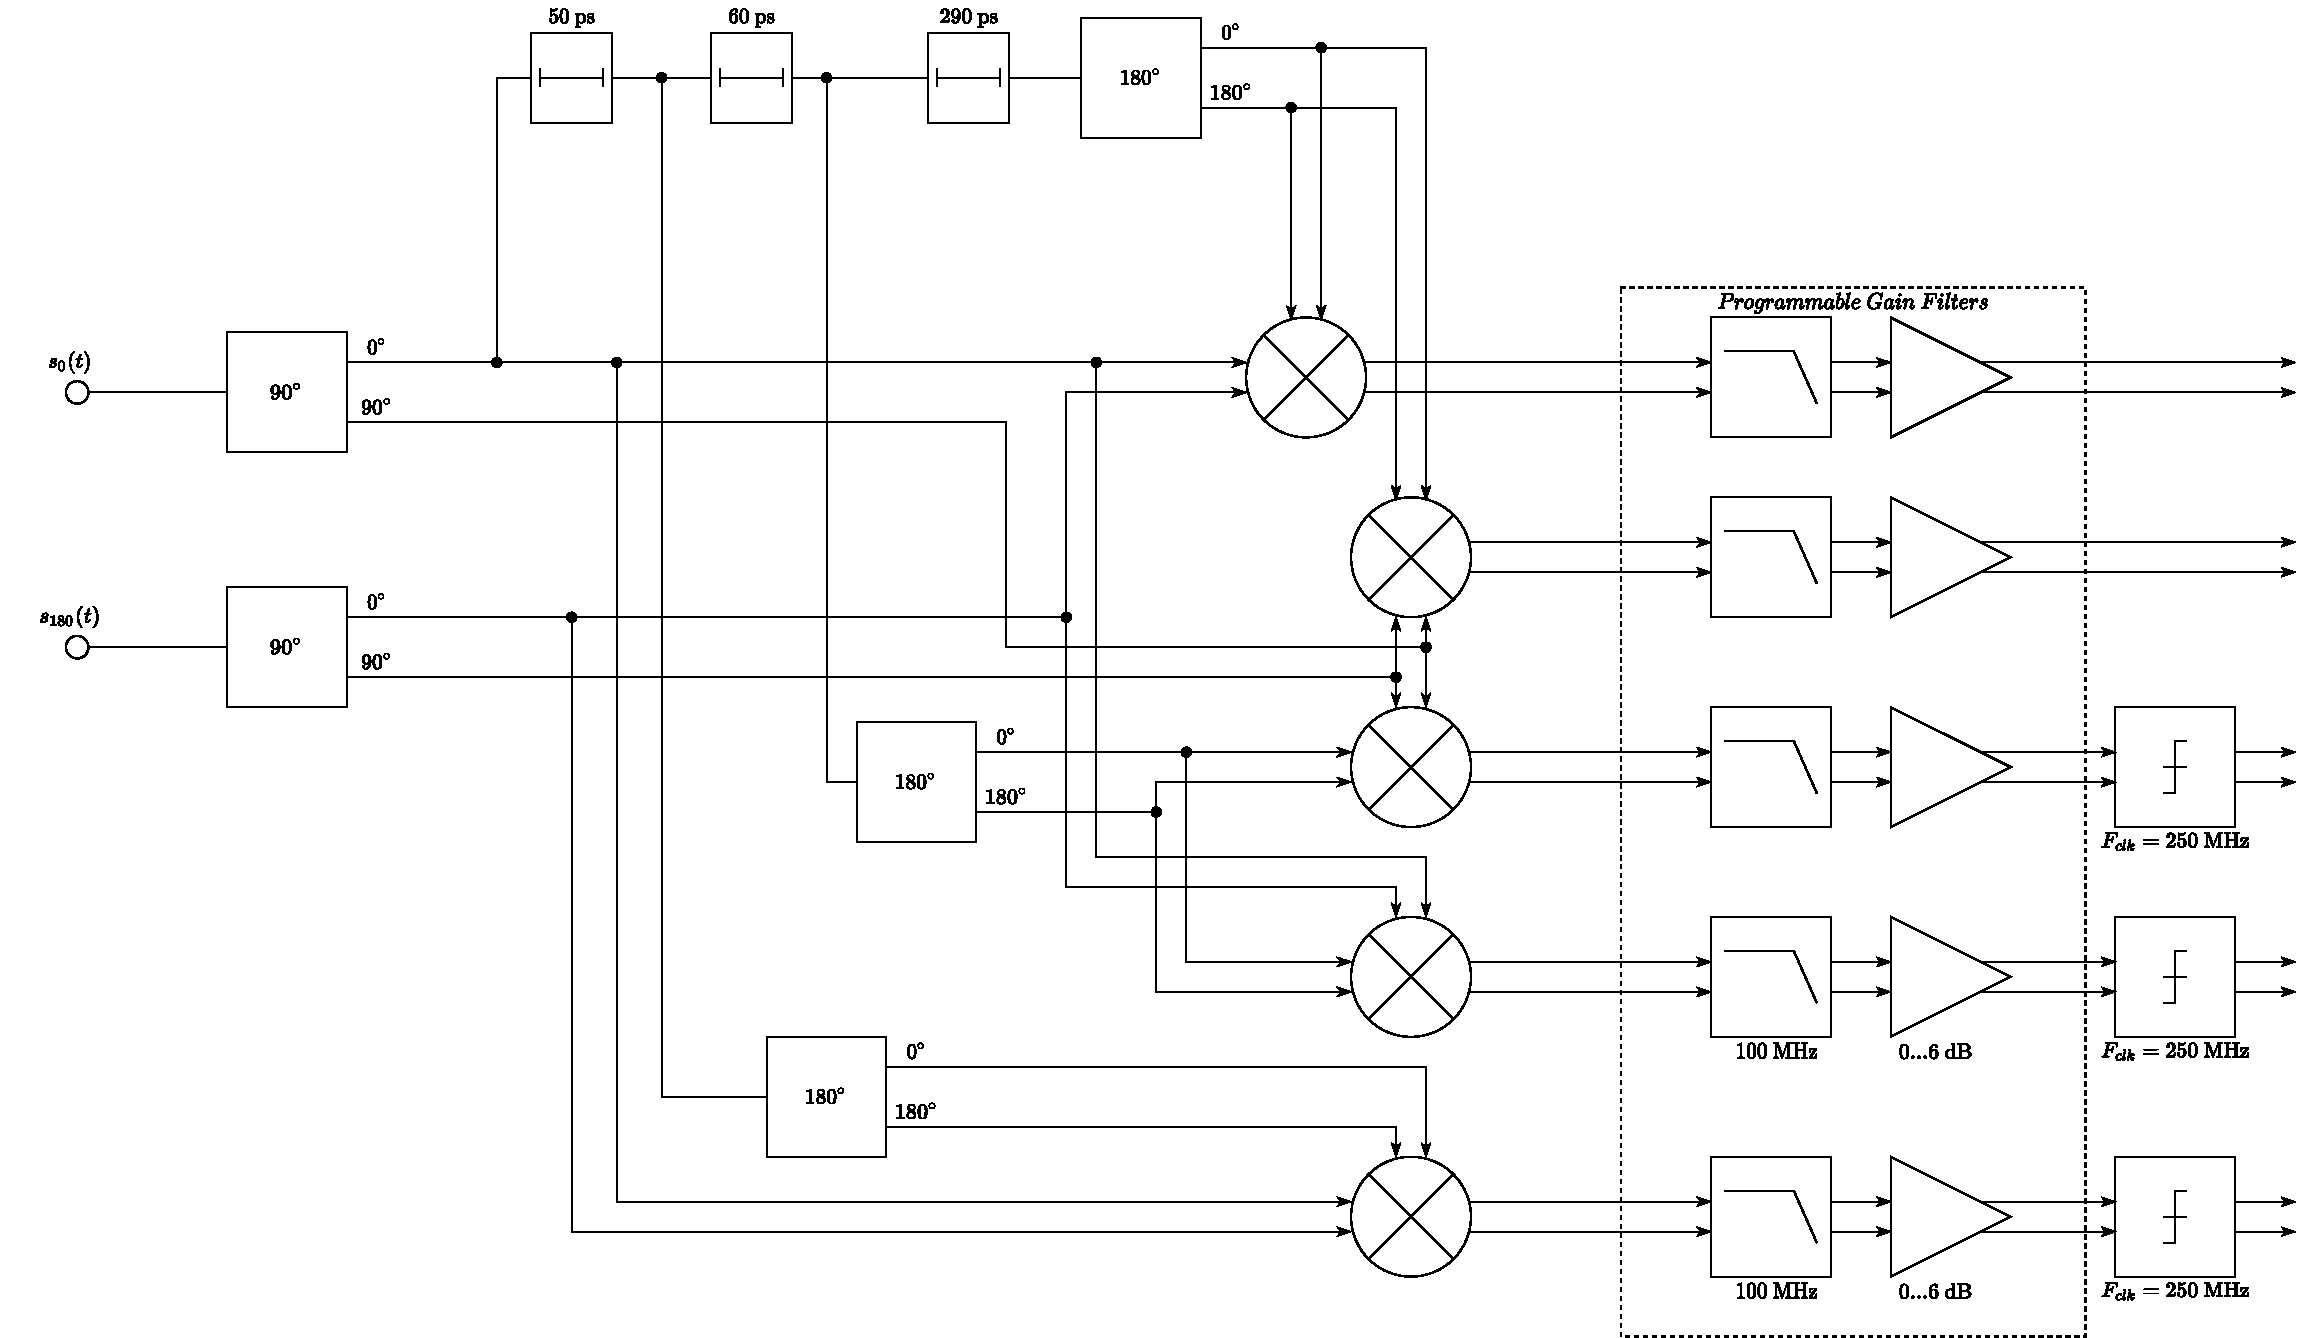
\includegraphics[width=1\linewidth]{IFM_Struct4.pdf}
	
	\caption{Структурная схема частотного дискриминатора диапазона \numrange{11.5}{18} ГГц}
	\label{ct:freq_estimate_11g5_18g}
\end{figure}

\begin{figure}[ht]
    \centerfloat{
        \hfill
        \subcaptionbox{\label{fig:ifm_1g_3g3}}{%
            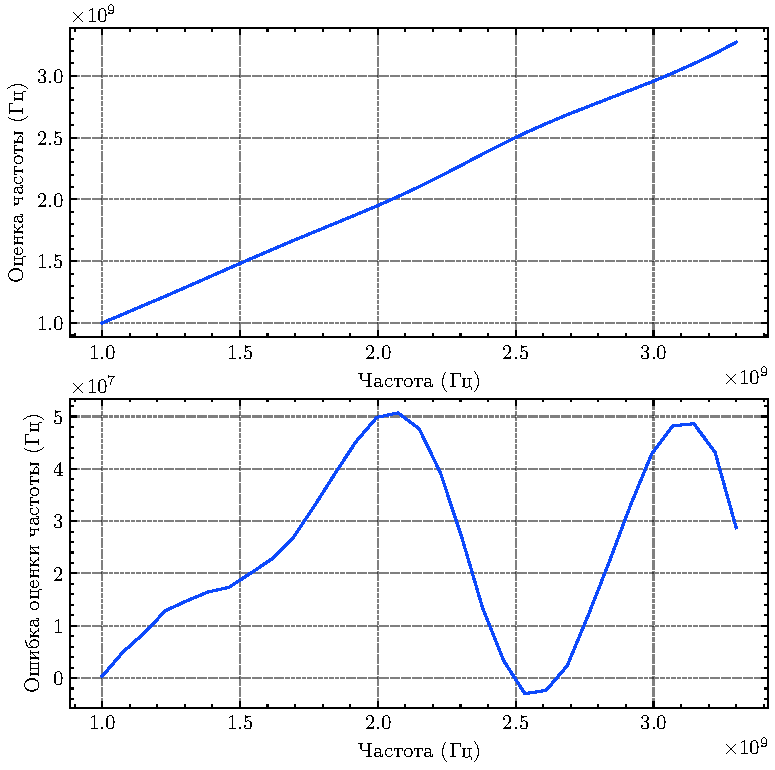
\includegraphics[width=0.45\linewidth]{ifm_1g_3g3.pdf}}
        \hfill
        \subcaptionbox{\label{fig:ifm_3g3_6g3}}{%
            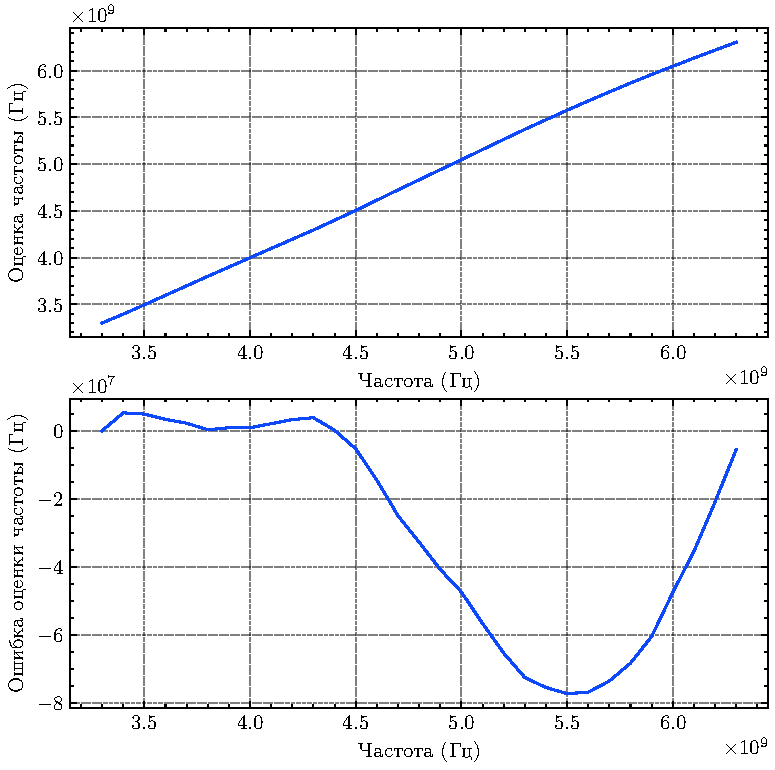
\includegraphics[width=0.45\linewidth]{ifm_3g3_to_6g3_27C.pdf}}
        \hfill
    }
	\centerfloat{
        \hfill
        \subcaptionbox{\label{fig:ifm_6g3_11g5}}{%
            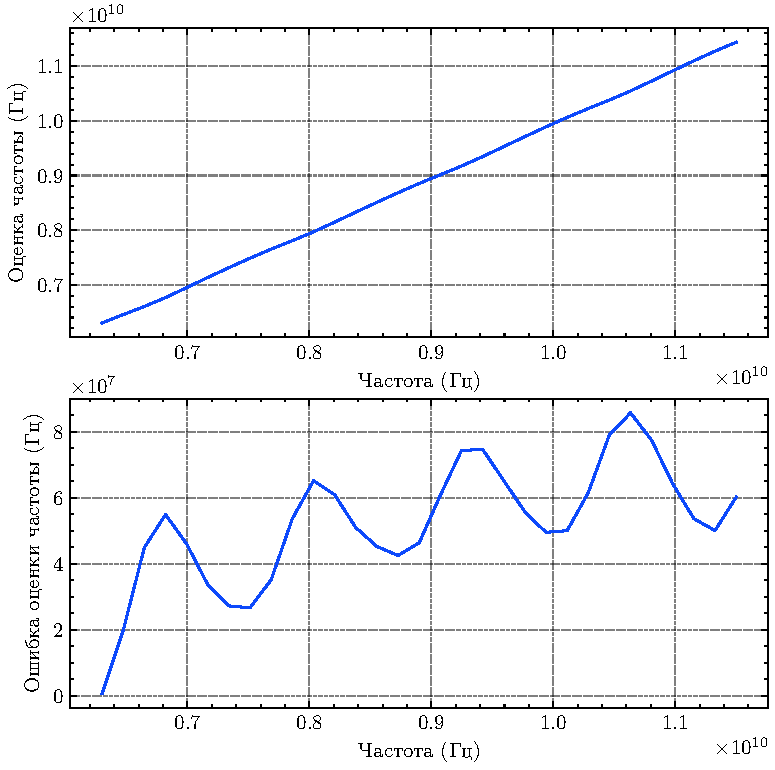
\includegraphics[width=0.45\linewidth]{ifm_6g1_to_11g5_27C.pdf}}
        \hfill
        \subcaptionbox{\label{fig:ifm_11g5_18g}}{%
            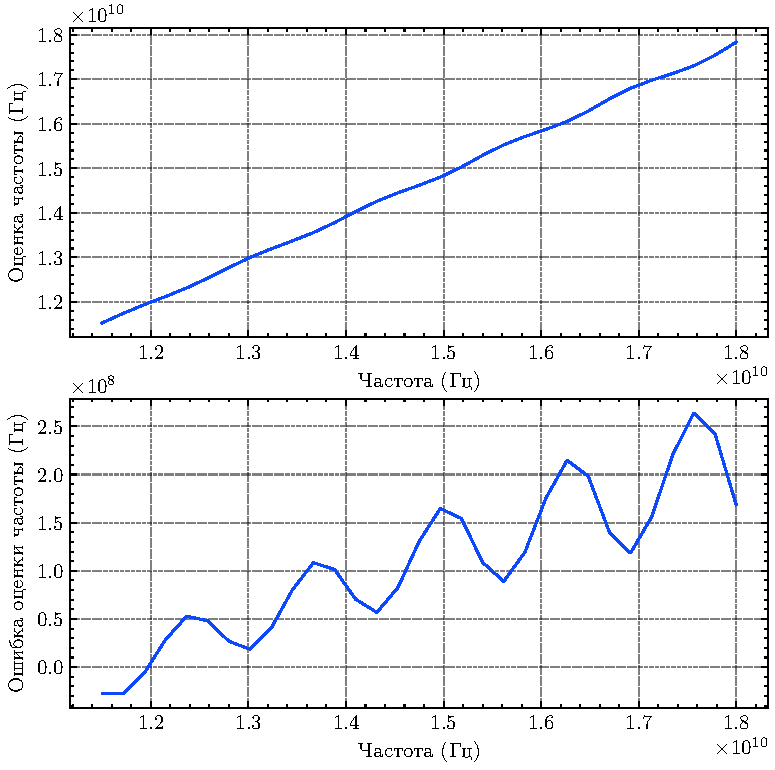
\includegraphics[width=0.45\linewidth]{ifm_11g5_to_18g_27C.pdf}}
        \hfill
    }
    \legend{а) \numrange[]{1}{3.3}~ГГц; б) \numrange[]{3.3}{6.3}~ГГц; в) \numrange[]{6.3}{11.5}~ГГц; г) \numrange[]{11.5}{18}~ГГц.}
    \caption[Результаты моделирования каналов МИЧ диапазона {\numrange[]{1}{18}~ГГц}]{Оценка частоты по результатам компьютерного моделирования каналов {\numrange[]{1}{18}~ГГц}}\label{fig:estimations_1g_18g}
\end{figure}

\section{Выводы по разделу}